\documentclass[twocolumn]{article}
\usepackage[english]{babel}
\usepackage[utf8]{inputenc}
\usepackage{amsmath,amssymb,physics,mathtools,blindtext,graphicx,float}
\usepackage[a4paper,total={7.5in,10in}]{geometry}
\usepackage[labelfont=bf]{caption}

\begin{document}
\begin{large}

\section*{Temperature of earth with idealized greenhouse model}
\subsection*{Introduction}
\begin{figure}[b!]
    \includegraphics[scale=0.5]{Layer1.png}
    \caption{}
    \label{11maj1748}
\end{figure}
In this report, an idealized greenhouse model is considered. The averaged flux density of the incoming solar radiation over the surface of the earth is $S_0 = 341.5$ Wm$^{-2}$, of which about $30$\% is reflected back into space. The average incoming radiation from the top of the atmosphere is thus $S = 0.7S_0 = 239.05$ Wm$^{-2}$. The atmosphere is to large extent transparent to this radiation and in this model it is assumed that all of this radiation reaches the surface of the earth. The surface of the earth, being much colder than the surface of the sun, emits radiation of much lower frequency back up into the atmosphere for which the atmosphere is much more opaque to.  The earth is considered to be in thermal equlibrium with its surrounding so that the net energy flux through the atmosphere is zero. In this model, the atmosphere is assumed to be divided into different layers acting as grey bodies with emissivity and absorptivity $\epsilon$ which means that the total energy flux emitted from a layer is equal to $\epsilon\sigma T^4$ where $T$ is the temperature of the layer and $\sigma$ is the Stefan-Boltzmann constant. The value of $\epsilon$ lies between zero and one. These layers are also assumed to be in a thermal equilibrium so that the total energy flux into each one of them equals the total energy flux out of them. Balancing the incoming and outgoing flux through the layers gives a system of equations which can be solved to give the temperature in each layer. This was done numerically for a different number of layers and the results were compared to measured data. 

\subsection*{One layer model}
The model described above can be understood as a generalization of a one-layer model of the atmosphere depicted in figure \ref{11maj1748}. As mentioned above, the incoming radiation from the sun $S$ does not directly affect the atmosphere layer but the radiation from the earth does. The temperature and emissivity of the surface are $T_0$ and $\epsilon_0$, respectively, and the temperature and emissivity of the atmosphere are $T_1$ and $\epsilon_1$. Zero net flux through layer 1 gives 
\begin{equation}
    \label{11maj2007}
    \begin{split}
        0 &= 2\epsilon_1\sigma T_1^4 + (1-\epsilon_1)\sigma T_0^4 - \epsilon_0\sigma T_0^4 \\ 
        &= 2\epsilon_1\sigma T_1^4 - \epsilon_0\epsilon_1\sigma T_0^4
    \end{split}
\end{equation}
and zero net flux through the top of the atmosphere gives 
\begin{equation}
    (1-\epsilon_1)\epsilon_0\sigma T_0^4 + \epsilon_1\sigma T_1^4 = S,
\end{equation}
These two equations are linear in $\sigma T_0^4$ and $\sigma T_1^4$ and can be easily solved to give a surface temperature of 
\begin{equation}
    \label{11maj2008}
    T_0 = \left(\frac{S}{\sigma(1-\epsilon_0\epsilon_1/2)}\right)^{1/4}.
\end{equation}

\subsection*{Multi-layer model}
The one-layer model can be generalized by adding more layers. For $N$ layers, the temperatures in the different layers $T_i$ will be given by the solution to the $N+1$ dimensional linear system of equations
\begin{equation}
    A\mathbf{x} = \mathbf{b}
\end{equation}
where $x_i = \sigma T^4_i$. The first row of $A$ corresponds to the equation of no net flux through the top of the atmosphere:
\begin{equation}
    \sum_{j=0}^{N}A_{0,j}x_j = S
\end{equation}
where $A_{0,j}x_j$ is the contribution of layer $j$ to this equation, i.e.
\begin{equation}
    A_{0,j}x_j = \epsilon_j(1-\epsilon_{j+1})(1-\epsilon_{j+2})\dots(1-\epsilon_{N})\sigma T_j^4.
\end{equation}
Row $i>0$ corresponds to the equation of no net flux through layer $i$. Its own contribution to this equation is
\begin{equation}
    A_{i,i}x_i = 2\epsilon_i\sigma T_i^4.
\end{equation}
It is then convenient to look at the contribution of layers $j<i$ and layers $j>i$ seperately. For $j<i$, the contribution from layer $j$ to the flux through layer $i$ is 
\begin{equation}
    \begin{split}
        A_{i,j}x_j &= \epsilon_j(1-\epsilon_{j+1})(1-\epsilon_{j+2})\dots(1-\epsilon_{i})\sigma T_j^4 \\ 
        &\hspace{0.3cm} -\epsilon_j(1-\epsilon_{j+1})(1-\epsilon_{j+2})\dots(1-\epsilon_{i-1})\sigma T_j^4 \\ 
        &= -\epsilon_i\epsilon_j(1-\epsilon_{j+1})(1-\epsilon_{j+2})\dots(1-\epsilon_{i-1})\sigma T_j^4.
    \end{split}
\end{equation}
The flux going out of layer $i$ is positive and the flux going into it is negative. For $j>i$, we have similarily
\begin{equation}
    \begin{split}
        A_{i,j}x_j &= \epsilon_j(1-\epsilon_{j-1})(1-\epsilon_{j-2})\dots(1-\epsilon_{i})\sigma T_j^4 \\ 
        &\hspace{0.3cm} -\epsilon_j(1-\epsilon_{j-1})(1-\epsilon_{j-2})\dots(1-\epsilon_{i+1})\sigma T_j^4 \\ 
        &= -\epsilon_i\epsilon_j(1-\epsilon_{j-1})(1-\epsilon_{j-2})\dots(1-\epsilon_{i+1})\sigma T_j^4.
    \end{split}
\end{equation}
The equation for zero net flux through layer $i$ is then
\begin{equation}
    \sum_{j=0}^{N}A_{i,j}x_j = 0.
\end{equation}
The vector $\mathbf{b}$ is thus given by $\mathbf{b} = (S,0,0,\dots,0)$. Having set up the matrix $A$ and vector $\mathbf{b}$, we could solve for the temperatures in each layer. However, the emissivities can depend on various physical variables such as temperature, density and wavelength of the radiation. Here, it will be assumed that the emissivities $\epsilon_j$ only depend on the densities of the layers $\rho_j$ and their thickness $h_j$ by the following relationship:
\begin{equation}
    \label{11maj1708}
    \epsilon_j = \alpha\rho_jh_j
\end{equation}
where $\alpha$ is a constant such that $0\leq\epsilon_j\leq 1$. The density of layer $j$ can be calculated from the ideal gas law and Boltzmann statistics:
\begin{equation}
    \label{11maj1959}
    \begin{split}
        &P_j = \rho_jk_BT_j/m \\ 
        &P_j = P_{j-1}e^{-mgh_{j-1}/k_BT_{j-1}}.
    \end{split}
\end{equation}
Here $P_j$ is the pressure in layer $j$, $k_B$ is the Boltzmann constant and $m$ is the average mass of an air molecule, $m=4.8\cdot 10^{-26}$ kg. Assuming a density dependence of the emissivity entails a complication however, because the density of air depends on its temperature, which is the variable we are trying to solve for. How this was solved is explained later. Assuming that we know $P_0$ and the temperature in each layer, we can calculate the density in each layer recursively with:
\begin{equation}
    \label{11maj1707}
    \rho_j = \frac{mP_{j-1}}{k_BT_j}e^{-mgh_{j-1}/k_BT_{j-1}},\quad j>0.
\end{equation}
This follows from equation \eqref{11maj1959}. The pressure and density at the surface are assumed to be $P_0=101.3$ kPa and $\rho_0=1.225$ kg/m$^3$, respectively.

Because of the temperature dependence of the emissivities, the system of equations becomes non-linear. Hence, it was solved iteratively until it became self-consistent with the following scheme: Some initial temperatures were chosen $T_j^{(0)}$ and the densities $\rho_j^{(0)}$ were found from them using equation \eqref{11maj1707}. Then, using these densities, the emissivities $\epsilon_j^{(0)}$ were found with equation \eqref{11maj1708}. New temperatures $T_j^{(1)}$ were then obtained as the solution to the linear system of equations $A(\mathbf{x}^{(0)})\mathbf{x}^{(1)} = \mathbf{b}$ where $A(\mathbf{x}^{(0)})$ is the matrix given above in which the emissivities $\epsilon_j^{(0)}$ were used. Then from the new temperatures, it was possible to obtain new densities $\rho_j^{(1)}$ and emissivites $\epsilon_j^{(1)}$. This was repeated until $|T_j^{(k)} -  T_{j}^{(k+1)}|$ became sufficiently small.
%The parameters of this model are the number of layers, $N$, and the emissivity of each layer $\epsilon_i$. The emissivities can depend on various physical variables such as temperature, density and wavelength of the radiation. If it is temperature dependent, the system of equations becomes non-linear.

\subsection*{Results}
\begin{figure}[!b]
    \begin{center}
        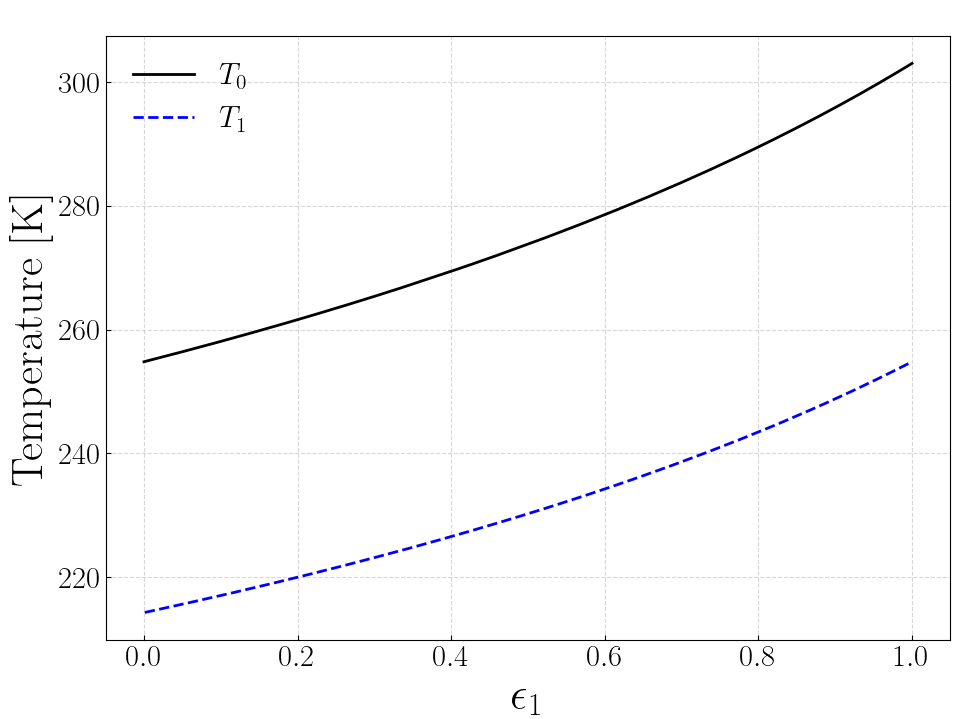
\includegraphics[scale=0.35]{OneLayer.png}
    \end{center}
    \caption{The surface temperature $T_0$ and the temperature of the atmosphere $T_1$ according to the one layer model, as a function of the emissivity of the atmosphere $\epsilon_1$.}
    \label{9maj1827}
\end{figure}
To begin with, the method was tested for one layer for which the solution is known analytically (eqs. \eqref{11maj2007}$-$\eqref{11maj2008}). The surface of the earth had emissivity $\epsilon_0=1$ and the emissivity of the atmosphere $\epsilon_1$ was varied between zero and one. The result can be seen in figure \ref{9maj1827}. The span of the surface temperature for different emissivities is $255-303$ K which at least contains the estimate for the surface temperature from measured data, $287.2$ K. The temperature in the atmosphere, $T_1$, is roughly $40-50$ K lower than $T_0$. This seemed to be a general characteristic of this model, i.e. that the higher layers always had lower temperature than the layers below. 
\begin{figure}[!t]
    \begin{center}
        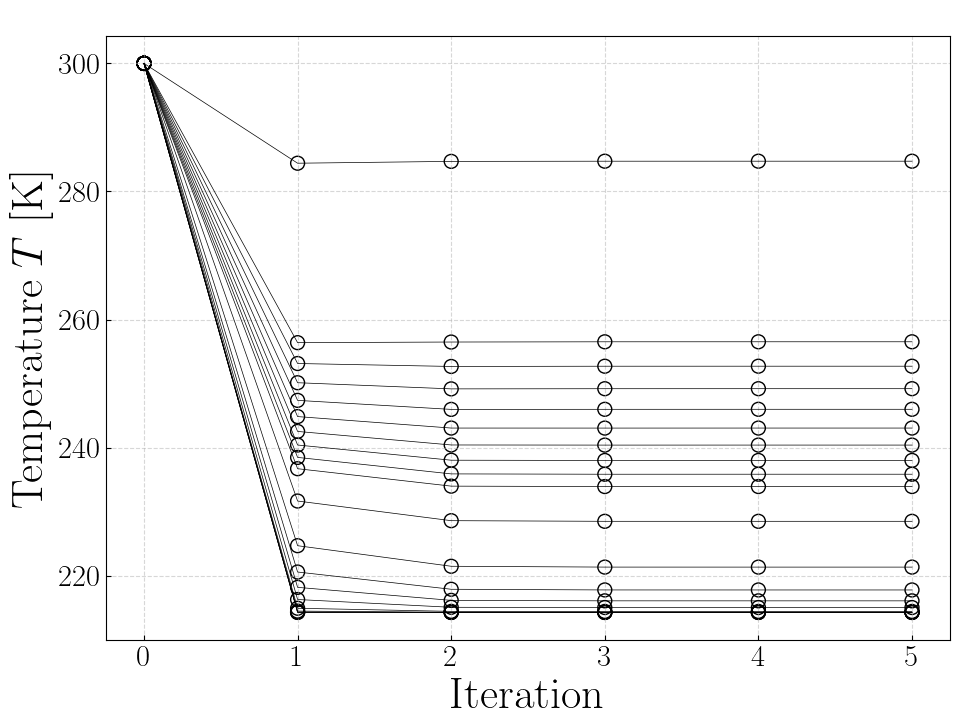
\includegraphics[scale=0.35]{Iteration.png}
    \end{center}
    \caption{The temperature as a function of iteration number when solving the system of equations for the multi-layer atmosphere model.}
    \label{9maj2056}
\end{figure}

Having tested the model for one layer, it was used on a multi-layer atmosphere where the emissivities depend on the densities according to equation \eqref{11maj1707}. Ten layers were placed between $z=0$ m and $z=10000$ m with $1000$ m spacing. Then four layers were placed between $z=10000$ m and $z=30000$ m with $5000$ m spacings. Lastly, six layers were placed between $z=30000$ and $z=90000$ with \mbox{$z=10000$ m} spacings. Hence, the model atmosphere extended to $z=90000$ m and was composed of twenty layers. The starting temperature for the iteration was $T_j^{(0)}=300$ K for all layers $j$. The constant $\alpha$ was chosen such that the surface temperature approximately matched the real surface temperature of the earth, $\alpha=1.2\cdot 10^{-4}$ m$^{2}$/kg (this is, admittedly, not very reasonable and reflects an aspect of what could be improved in the model, i.e. how the emissivities of different layers of the atmosphere are estimated). The temperature in each layer as a function of iteration number can be seen in figure \ref{9maj2056}. The temperatures converge rather quickly. The converged values of the temperatures as a function of alititude $z$ can be seen in figure \ref{9maj2055}. A similar plot for the density can be seen in figure \ref{9maj2054}. 

As a reference, the temperatures and densities from the US standard atmosphere model from 1976 are also plotted. The similarity is the sharp decrease in temperature for the first $\approx 15000$ m. In the multi-layer model, however, the temperature is a decreasing function of altitude, and cannot explain the increase of temperature with altitude which is observed in the atmosphere of the earth. The density, on the other hand, agrees quite well with the density of the earth. 
\begin{figure}[!t]
    \begin{center}
        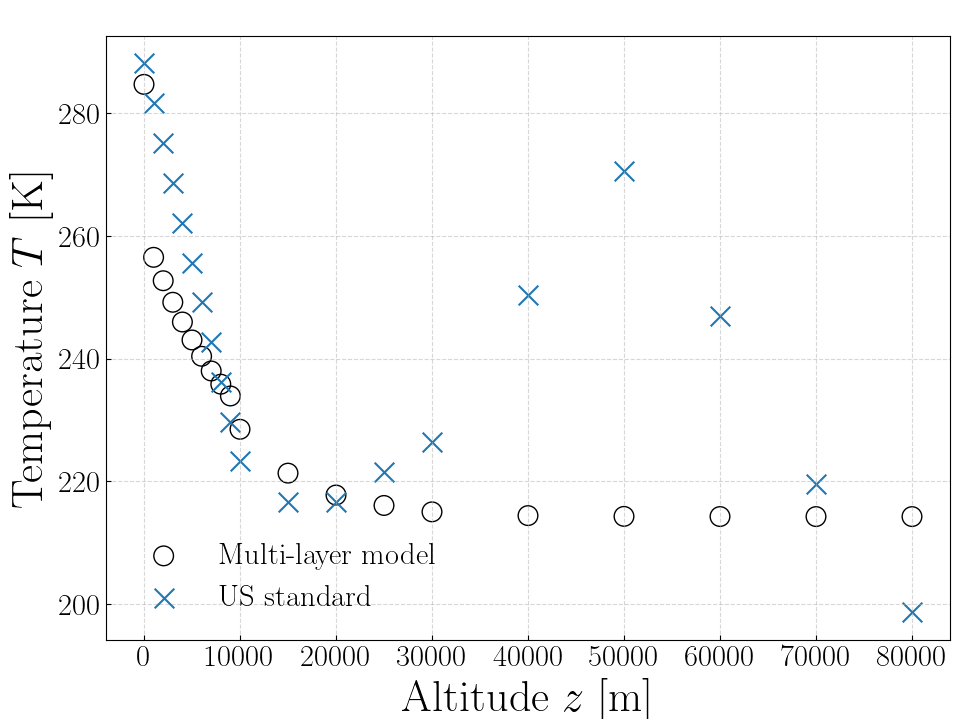
\includegraphics[scale=0.35]{Temperature.png}
    \end{center}
    \caption{The temperature as a function of altitude obtained with the multi-layer model of the atmosphere. The values according to the US standard atmosphere model is plotted for comparison.}
    \label{9maj2055}
    \begin{center}
        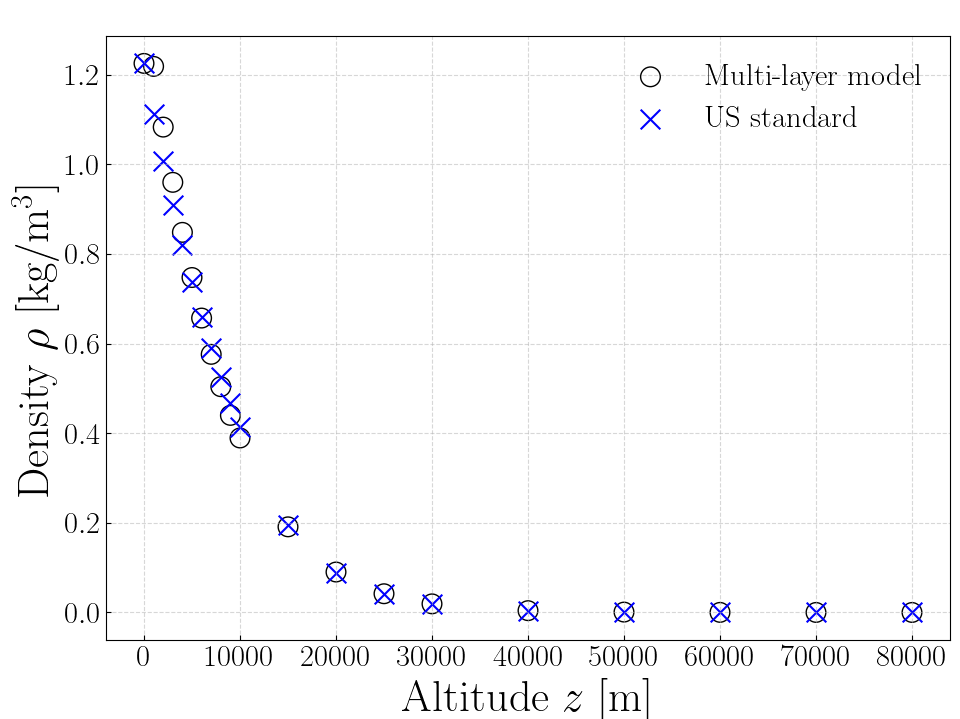
\includegraphics[scale=0.35]{Density.png}
    \end{center}
    \caption{The density as a function of altitude obtained with the multi-layer model of the atmosphere. The values according to the US standard atmosphere model are also plotted.}
    \label{9maj2054}
\end{figure}



























%\begin{equation*}
%    \begin{split}
%        &T_i^\text{Vi,In} = T_{i+1}^\text{Vi,In}e^{-\sigma_\text{Vi}\rho_ih} \\ 
%        &T_i^\text{IR,In} = \left(T_{i+1}^\text{In,IR}+\frac{E_{i+1}}{2}\right)e^{-\sigma_\text{IR}\rho_ih} \\ 
%        &T_i^\text{Out} = \left(T_{i-1}^\text{Out}+\frac{E_{i-1}}{2}\right)e^{-\sigma_\text{IR}\rho_ih} \\ 
%        &E_i = \left(\frac{E_{i-1}+E_{i+1}}{2}+T^\text{Out}_{i-1}+T^\text{IR,In}\right)\left(1-e^{-\sigma_\text{IR}\rho_ih}\right) \\ 
%        &\hspace{5.2cm} + T_{i+1}^\text{Vi,In}\left(1-e^{-\sigma_\text{Vi}\rho_ih}\right)
%    \end{split}
%\end{equation*}
%Given an initial condition $T_N^\text{Vi,In}$, we can easily calculate all other $T_i^\text{Vi,In}$ if we know $\rho_i$. The other three equations can be written as 
%\begin{equation}
%    \begin{split}
%        &T_i^\text{IR,In} - g_iT_{i+1}^\text{IR,In}-\frac{g_i}{2}E_{i+1} = 0 \\ 
%        &T_i^\text{Out} - g_iT_{i-1}^\text{Out} - \frac{g_i}{2}E_{i-1} = 0\\ 
%        &E_i - \frac{1-g_i}{2}E_{i-1} - \frac{1-g_i}{2}E_{i+1} \\ 
%        &\hspace{0.4cm} - (1-g_i)T^\text{Out}_{i-1} - (1-g_i)T^\text{IR,In}_{i+1} = b_i
%    \end{split}
%\end{equation}
%where 
%\begin{equation}
%    \begin{split}
%        &g_i = e^{-\sigma_\text{IR}\rho_ih}, \\ 
%        &b_i = T_{i+1}^\text{Vi,In}\left(1-e^{-\sigma_\text{Vi}\rho_ih}\right).
%    \end{split}
%\end{equation}
%This system of equations can be solved given initial conditions $T^\text{IR,In}_N$, $T^\text{Out}_N$ and $E_N$ if $\rho_i$ is known.






\end{large}
\end{document}
